\documentclass[a4paper]{article}
\usepackage[warn]{mathtext}
\usepackage[utf8]{inputenc}
\usepackage[T2A]{fontenc}
\usepackage[english,russian]{babel}
\usepackage{multicol}
\usepackage{fancyhdr}
\usepackage{graphicx}
\usepackage{microtype}
\usepackage{wrapfig}
\usepackage{amsmath}
\usepackage{floatflt}
\usepackage{geometry} \geometry{verbose,a4paper,tmargin=2cm,bmargin=2cm,lmargin=1.5cm,rmargin=1.5cm}
\usepackage{float}
\usepackage{amssymb}
\usepackage{caption}
\usepackage{epsfig}
\usepackage{newunicodechar}

\begin{document}

\graphicspath{ {pictures/} }

\begin{titlepage}
	\centering
	\vspace{5cm}
    {\scshape\LARGE Московский физико-технический институт\par}
	\vspace{5cm}
	{\scshape\Large Лабораторная работа по общей физике \par}
	\vspace{1cm}
    {\huge\bfseries  4.1 Определение энергии $\alpha$-частиц по величине их
    пробега в воздухе \par}
	\vspace{1cm}
	\vfill
    \begin{flushright}
        {\large выполнил студент Б04-852 группы ФЭФМ}\par
        \vspace{0.3cm}
        {\LARGE Яромир Водзяновский}
    \end{flushright}
	\vfill
Долгопрудный, 2020
% Bottom of the page
\end{titlepage}

\pagestyle{fancy} 
\fancyhead[L]{$\alpha$-частицы    $\sim  \hat(\, ^{\circ}  \omega  ^{\circ} \, \hat) \sim$}
\fancyhead[R]{Квантовая физика}
\fancyhead[C]{}
\fancyfoot[C]{ \noindent\rule{\textwidth}{0.4pt} \thepage }

\tableofcontents

\newpage



\section{Цель работы}

\begin{itemize}
    \item Измерить пробег $\alpha$-частиц в воздухе с помощью счетсчика Гейгера
    \item Измерить пробег $\alpha$-частиц в воздухе с помощью ионизационной камеры
    \item Определить энергию частиц
\end{itemize}



\section{Теория}

При $\alpha$-распаде исходное родительское ядро яспускает ядро гелия и превращается в дочернее ядро,
число протонов и нейтронов уменьшается на 2 единицы. Вариьрование периодов полу распада велико для 
$_{84}^{212}Po$ составляет $3 \cdot 10^{-7} \; c$, а для $_{82}^{204}Pb$ составляет $1.4 \cdot 10^{17} \; лет$. 
Диапазон изменения энергии вылетающей $\alpha$-частицы - от 4 до 9 МэВ, причем, чем меньше энергия, 
тем больше период полураспада. Связь между энергией $\alpha$-частицы $E$ и периодом полураспада ядра
$T_{1/2}$:

\begin{equation}
    \lg{T_{1/2}} = \frac{a}{\sqrt{E}} + b,
\end{equation}

получена экспериментально Х.Гейгером и Дж. Нэттолом в 1911 г. \par 

Вероятность вылета $\alpha$-частицы из ядра определяется вероятностью ее проникновения сквозь кулоновский барьер.
Экспоненциальный характер обусловлен экспоненцианльным затуханием волновой функции в области под 
барьером, где $\Pi > E$. \par

Экспериментально будем опредлять энергию $\alpha$-частиц по величине  их пробега в веществе.
Тяжелые частицы с $Z = 1, 2$ при прохождении в веществе теряют  свою энергию в неупругих столкновениях 
с атомами вещества, что вызывает \textbf{ионизацию и возбуждение}, поэтому такие потери называют \textbf{ионизационными}.
Энергия передаваема электрону не превышает $4mE/M$, где $m$ - масса электрона, $M$ - масса заряженной частицы,
$E$ - кинетическая энергия заряженной частицы. Угол отклонения $m/M$ мал (потеря энергии 1/2000), 
значит трактория прямолинейна. \par

В нашем случае идут процессы до 10 МэВ. Ядерные взаимодействия имеют весомый вклад при выских энергиях, 
когда энергия вылетающих $\alpha$-частиц выше кулоновского барьера. в нашем случае это не так и 
почти весь вклад в потери вносяит непругое взаимодействие. \par 

Произведем расчет удельных потерь энергии. Пусть частица с зарядом $z$ движется в направлении $x$ 
и проходит на расстоянии $y$ от электрона. Атомные электироны считаем свободными ввиду большгой энергии 
налетающих частиц. В таких условиях элекрону передается только импульс в перпендикулярном напралвении,
который равен произведению электростатической силы $Z e^2 / y^2$ на время $\approx 2y/v$. Значит приобритенная 
энергия $E_e$:

\begin{equation}
    E_e = \frac{p^2}{2m} = \frac{1}{2m} \left ( \frac{Ze^2}{y^2} \cdot \frac{2y}{v} \right )^2 = \frac{2 e^4 Z^2}{mv^2y^2}
\end{equation}

Если плотность электронов в среде $n_e = nZ$ ($n, \; Z$ - плотность атомов среды и заряж соотв.), то потери
энергии заряженной частицы на единице пути в результате взаимодействия с электронами в слое $2 \pi y dy$:

\begin{equation}
    dE(y) = \frac{4 \pi n Z z^2 e^4}{mv^2} \cdot \frac{dy}{y}
\end{equation}

Проинтегрировав выражение выше получим потерю энергию на единице пути:

\begin{equation}
    \left ( \frac{dE}{dx} \right )_{ион} \approx 4\pi \frac{e^4 z^2}{mv^2} n Z \ln{\frac{y_{max}}{y_{min}}}
\end{equation}

Найдем пределы $y_{max}$ и $y_{main}$, из (2) следует, что энергия, потерянная заряженной частицой
при столкновении с электроном обратно пропорциональна квадрату прицельного параметра:

\begin{equation}
    2 \ln{\frac{y_{max}}{y_{min}}} = - \ln{\frac{E_{max}}{E_{min}}}
\end{equation}

Из ЗСЭ:

\begin{equation}
    E_{max} = \frac{4mE}{M} = 2 mv^2
\end{equation}

В системе покоя частицы электрон может отскочить от нее и изменить скорость на $2 v$. Минимальная энергия, 
передаваема электрону в случае связанных электронов определяется жнергией связи или энергией возбуждения. Для определенного вида атомов 
или молекул это минимальное значение потерянной энергии называется \textbf{средним ионизационным потенциалом} $\bar{I}$:

\begin{equation}
    \ln{\frac{E_{max}}{E_{min}}} = \ln{\frac{2mv^2}{\bar{I}}}
\end{equation}

Для ионизационных потерь нерелятивистской тяжелой заряженной частицы:

\begin{equation}
    \left ( \frac{dE}{dx} \right )_{ион} \approx 2 \pi \frac{e^4 z^2}{mv^2} n Z \frac{2mv^2}{\bar{I}}
\end{equation}

Величину $dE/dx$ называют тормозной способностью вещества. \par 

\begin{wrapfigure}[14]{r}{130pt}
    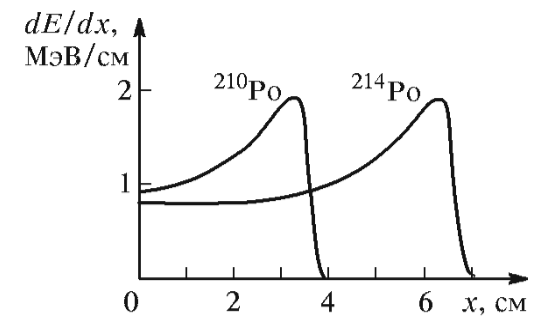
\includegraphics[scale = 0.6]{picbreg.png}
    \caption{Кривые Брэгга для $\alpha$-частиц}
    \label{ris breg}
\end{wrapfigure}

В формулу (8) входит только скорость и заряд частицы. С увеличением скорости потери уменьшаются.\par 

Зависимость $dE/dx$ от пути есть кривая Брэгга на рис. \ref{ris breg}. Путь тяжелых зарженных частиц прямолинеен, 
а разброс длин путей от многократного кулоновского рассеяния невелик, так что можно говорить о длине пробега заряженных частиц 
в веществе. \par 

Зная зависимост тормозной способности данного вещества от жнергии частицы можно вычяислить длину пробега частицы, замедляющейся 
от начальной жнергии $E_0$ до $E_1$. Длину пробега частицы с зарядом $z$ и массой $M$ в веществе с атомным номером $Z$ :

\begin{equation}
    R_{zM} = - \int\limits _{E_1}^{E_0} \frac{dE}{(dE / dx)} = \frac{m}{2 \pi e^4 z^2 n Z} \int\limits_{E_1}^{E_0} \frac{v^2 dE}{\ln{(2mv^2/\bar{I})}}
\end{equation}

Примем во внимание, что $dE = Mvdv$:

\begin{equation}
    R_{zM} = \frac{m M}{2 \pi e^4 z^2 n Z} \int\limits_{v_1}^{v_0} \frac{v^3 dv}{\ln{(2mv^2/\bar{I})}}
\end{equation}

Пренебрежом слабой логарифмической зависимостью от скорости частиц:

\begin{equation}
    R \propto \frac{M}{z^2} v_0^4 \propto E^2
\end{equation}

Однако эта формула плохо работает на экспериментальных данных. Получить хорошее согласие при учете взаимодействия только с
электронами не удается. Поэтому пользуются эмпирическим соотношением между энергией альфа-частицы и ее пробегом.
В диапазоне от 4 до 9 МэВ эта связь хорошо описывается выражением:

\begin{equation}
    R = 0.32 E^{3/2}
\end{equation}

Пробег выражается в сантиметрах, а энергия в МэВ. \par 

Формула (8) показщывает, что потери жнергии пропорциональны произведению плотности электронов на длину пути:
$\Delta E \propto n_e \Delta x$. В заданной среде плотность электронов пропорциональна обычной плотности.

\begin{equation}
    n_e = \rho N_A Z/A,
\end{equation}

$N_A$ - постоянная Авогадро, А - атомная масса вещества, Z - атомный номер. Иными словами удобнее понимать произведение 
плотности среды на пробег $R' = \rho \cdot R$ имеет размерность $г/см^2$. 

\begin{wrapfigure}[14]{r}{130pt}
    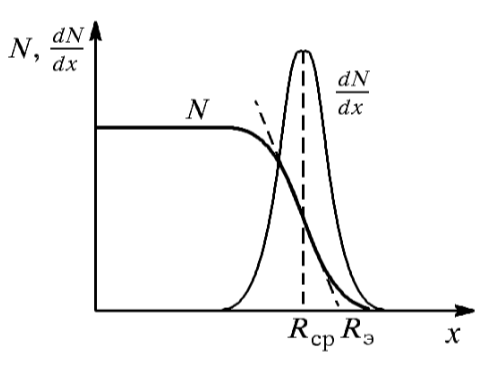
\includegraphics[scale = 0.6]{number.png}
    \caption{Зависимость числа $\alpha$-частиц от глубины их проникновения в вещество}
    \label{ris number}
\end{wrapfigure}

Рассеяние альфа-частиц имеет статистический характер. Кривая на рис. \ref{ris number} выражает зависимостьчисла частиц 
от расстояния, пройденного в поглотителе. \par 

Как видно из рис. \ref{ris number} $dN/dx$, большая часть альфа-частиц останавливается в узкой области, расположенной около 
$R_{ср}$, именно этот средний пробег входит в формулу (12). Однако, можно вместо среднего пробега использовать экспраполируемый 
$R_э$ - есть пересечение касательной, проходящей через перегиб, с абсциссой. \par

Несмотря на наличие коллиматора мы имеем дело с не с узкими параллельными пучками, а с пучками конечных размеров, так что есть заметная 
угловая расходимость. Это значит, что экспериментально зависимости числа альфа-частиц от глубины их проникновения передают проявление 
брэгговского пика и относительную величину пробега частиц с разной энергией. Однако пик оказывается размыт, так что будем пользоваться экстраполируемым пробегом. \par 

При эксперименталном исследовании проьега альфа-частиц следует помнить, что источники чатиц могу загрязнять 
близлежащие поверхност. Это происходит из-за отдачи, которую испытывают атомы при испускании альфа-частиц. Поэтому 
источники покрывают пленкой, которая все же замедляет частицы. \par 

В качестве источника используется $^{239}Pu$ с периодом полураспада $T_{1/2} = 2.44 \cdot 10^4 \;  лет$. 
Средняя энергия $5.15$ МэВ.



\section{Лабораторгная установка}



\subsection{Счетсчик Гейгера}

\begin{wrapfigure}[14]{l}{130pt}
    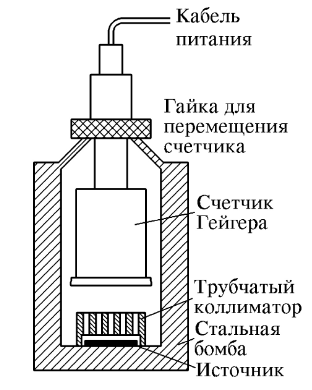
\includegraphics[scale = 0.7]{risgeyger.png}
    \caption{Схема торцевго счетсвика Гейгера}
    \label{ris geyger}
\end{wrapfigure}

Для определения пробега альфа-частиц с помощью счетчика радиоактивный источник помещается на дно стальной цилиндрической бомбы
(рис. \ref{ris geyger}), в которой может перемещаться торцевой счетчик Гейгера. Его
чувствительный объем отделен от наружной среды тонким слюдяным
окошком, сквозь которое могут проходить альфа-частицы. Рабочее напряжение счетчика указано на установке. \par  

Импульсы, возникающие в счетчике, усиливаются и регистрируются пересчетной схемой. Путь частиц в воздухе зависит от расстояния между источником и счетчиком. Перемещение счетчика производится путем вращения гайки, находящейся на крышке бомбы. Расстояние
между счетчиком и препаратом измеряется по шкале, нанесенной на
держатель счетчика. Счетчик не может быть придвинут к препарату ближе чем на 10 мм, т. к. между источником и счетчиком установлен коллиматор, изготовленный из плотно сжатых металлических трубок. Отверстия трубок пропускают к счетчику только те альфа-частицы, которые вылетают из источника почти перпендикулярно его поверхности.

\
\

\subsection{Ионизационная камера}

Ионизационная камера - прибор для количественного измерения ионизации, произведенной заряженными частицами 
при прохождении через газ. Камер - сосуд, наполенный газом с двумя электродами (рис. \ref{ris ioncam}).

\begin{wrapfigure}[19]{l}{180pt}
    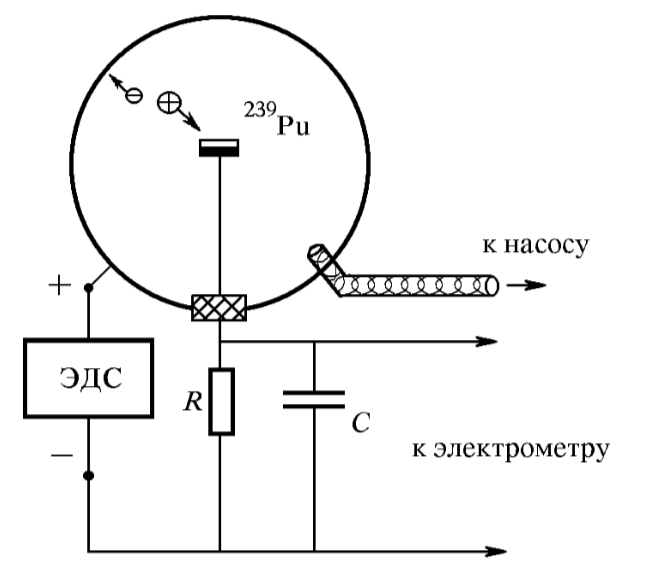
\includegraphics[scale = 0.6]{risioncam.png}
    \caption{Схема устройства ионизационной камеры}
    \label{ris ioncam}
\end{wrapfigure}

Сферическая стенка - электрод, второй электрод вводится в газ через изолюрующую пробку.
К электродам подводится постоянное напряжение от ЭДС. \par 

Газ сам по себе не проводит ток, он может проводить когда проходящая заряженная частица 
ионизирует газ при пролете. \par 

Поместим на торец внутреннего электрода источник $\alpha$-частиц $_{94}^{239}Pu$, заполним обьем камеры воздухом 
и начнем постепенно уеличивать разность потенциалов между электродами. Ток, протекший через камеру, вначале будет возрастать,
потом с некоторого напяржения $V_0$ станет постоянным (рис. \ref{vax}). Предельный ток будет равен $I_0 = n_0 \cdot e$, 
где $n_0$ - число пар ионов, образуемых в секунду в обьеме камеры. \par 

При небольших напряжениях сила тока меньше предельной, так как ионы успевают рекомбинировать и не дозодят до 
камеры. При напряженяих порядка сотен вольт почти ве ионы долетают. \par 

Прохождение тока через камеру регистрируется измерением напряжения на сопротивлении $R$. 
Так как средняя энергия ионизации воздуха около 30 кэВ, то альфа-частица с энергией 3 МэВ образует на своем пути 
около 100000 электронов с зарядом $1.6 \cdot 10^{-14}Кл$. Чтобы такой маленький заряд вызвал измеряемое напряжение
емкость $C$ должна быть мала. 

\begin{figure}[h]
    \begin{center}
    \begin{minipage}[h]{0.3\linewidth}
    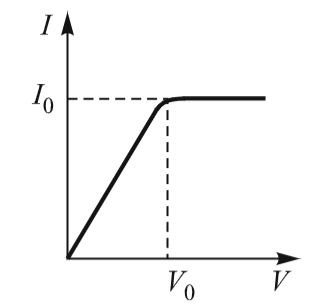
\includegraphics[width=1\linewidth]{vax.png}
    \caption{ВАХ ионизационной камеры} 
    \label{vax}
    \end{minipage}
    \hfill 
    \begin{minipage}[h]{0.3\linewidth}
    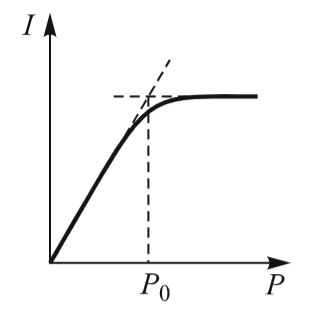
\includegraphics[width=1\linewidth]{iotp.png}
    \caption{Характерная кривая зависимости тока ионизационной камеры от давления}
    \label{iotp}
    \end{minipage}
    \end{center}
\end{figure}

Подвижность электронов в 1000 раз больше подвижности ионов. Подбором параметров $RC$ - цепочки
можно выделить импульсы тока соответсвующие только электронной компоненте. Реальное время несколько микросекунд. \par 

Если число прошедших через камеру альфа-частиц велико, то можно регистрировать ток, который пропорционален 
интенсивности альфа-частиц. Постоянная времени равна несокльким секундам. \par 

При изменении давления ионизационный ток будет меняться согласно рис. \ref{iotp}. При небольших энергиях газа 
альфа-частицы передают часть энергии стенкам камеры. При достижении $P_0$ все частицы заканчивают свой пробег внутри газа и рост тока прекращается. \par

В данной раьботе внутренний электтрод есть диск диаметром 5 мм, на который нанесен тонким слоем $_{94}^{239}Pu$, покрытый сверху тонкой защитной пленкой.
Второй электирод - волый шар с диаметром 100 мм. Разность потенциалов составляет 300 В. Установка содержит кран и манометр. 
Величина тока ионизации измеряется электрометром из сопротивлений $R = 100 МоМ$ (C = $10^{-8}$ Фарад , так что $RC = 1c$ )



\subsection{Сцинтилляционный счетсчик}

Установка состоит из цилиндрической камеры, на дне которой находится препарат. Камера закрыта стеклянной пластинкой,
на которую с двух сторон нанесен люминофор, с наруэной стороны к стеклу прижэат фотокатод фотоумножителя (рис. \ref{scin})

\begin{figure}[H]
    \begin{center}
    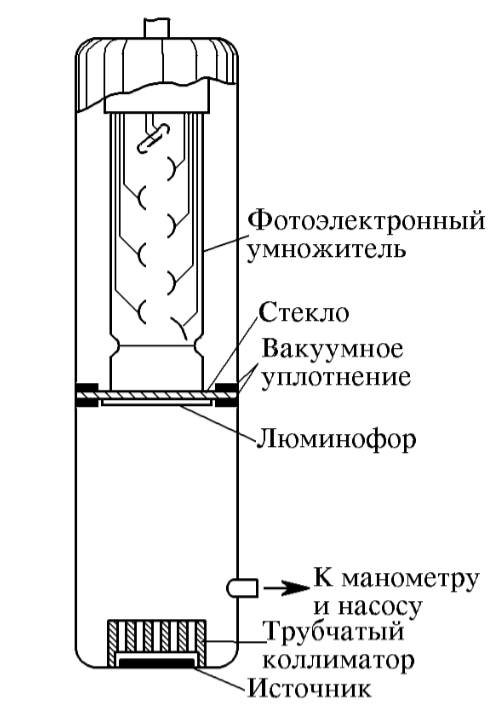
\includegraphics[scale = 0.8]{scin.png}
    \caption{Устанвока для измерения пробега с помощью сцинтилляционного счетсчика}
    \label{scin}
    \end{center}
\end{figure}
 
Оптичесмкий контакт ФЭУ-стекло обеспечивается тонким слоем вазелинового масла. Сигналы с фотоумножителя поступают на пересчетную устанвок. 
расстояние между препаратом и люминофором составляет 9 см, так что альфа-частицы не могут достигнуть 
люминофора. Будем определять зависимость интенсивности счета от давления в камере. 


\section{Ход работы}


\subsection{Счетсчик Гейгера}

\begin{enumerate}
    \item Включим устанвоку и высоковольтный выпрямитель, прогреем их. 
    

    \item Пока установка прогревается протестируем ее: при необходимом напряжении на счетсчике измерим
    счет при >4 см и при минимальном расстоянии счетсчика от источника, получим, что есть отличающийся счет.


    \item Проведем измерения зависимости счета от расстояния, результат занесем в таблицу 1. Расчитаем скорость счета $N_1$ разделив $N$
    на время измернеия 60 секунд.
    
    \begin{table}[h]
        \centering
        \caption{}
        \label{t1}
        \begin{tabular}{|c||c|c|c|c|c|c|c|c|c|c|c|}
            \hline
            x, мм&10&11&12&13&14&15&16&17&18&19&20 \\ \hline
            N&860&856&880&885&856&847&888&702&190&18&13 \\ \hline
            $N_1$, $c^{-1}$&14&14&14&15&14&14&15&12&3&0&0 \\ \hline
   
        \end{tabular}
    \end{table}


    \item Построим по данным из таблицы 1 график $N_1 = N_1(x)$ на рис. \ref{gr1}

    \begin{figure}[H]
        \begin{center}
        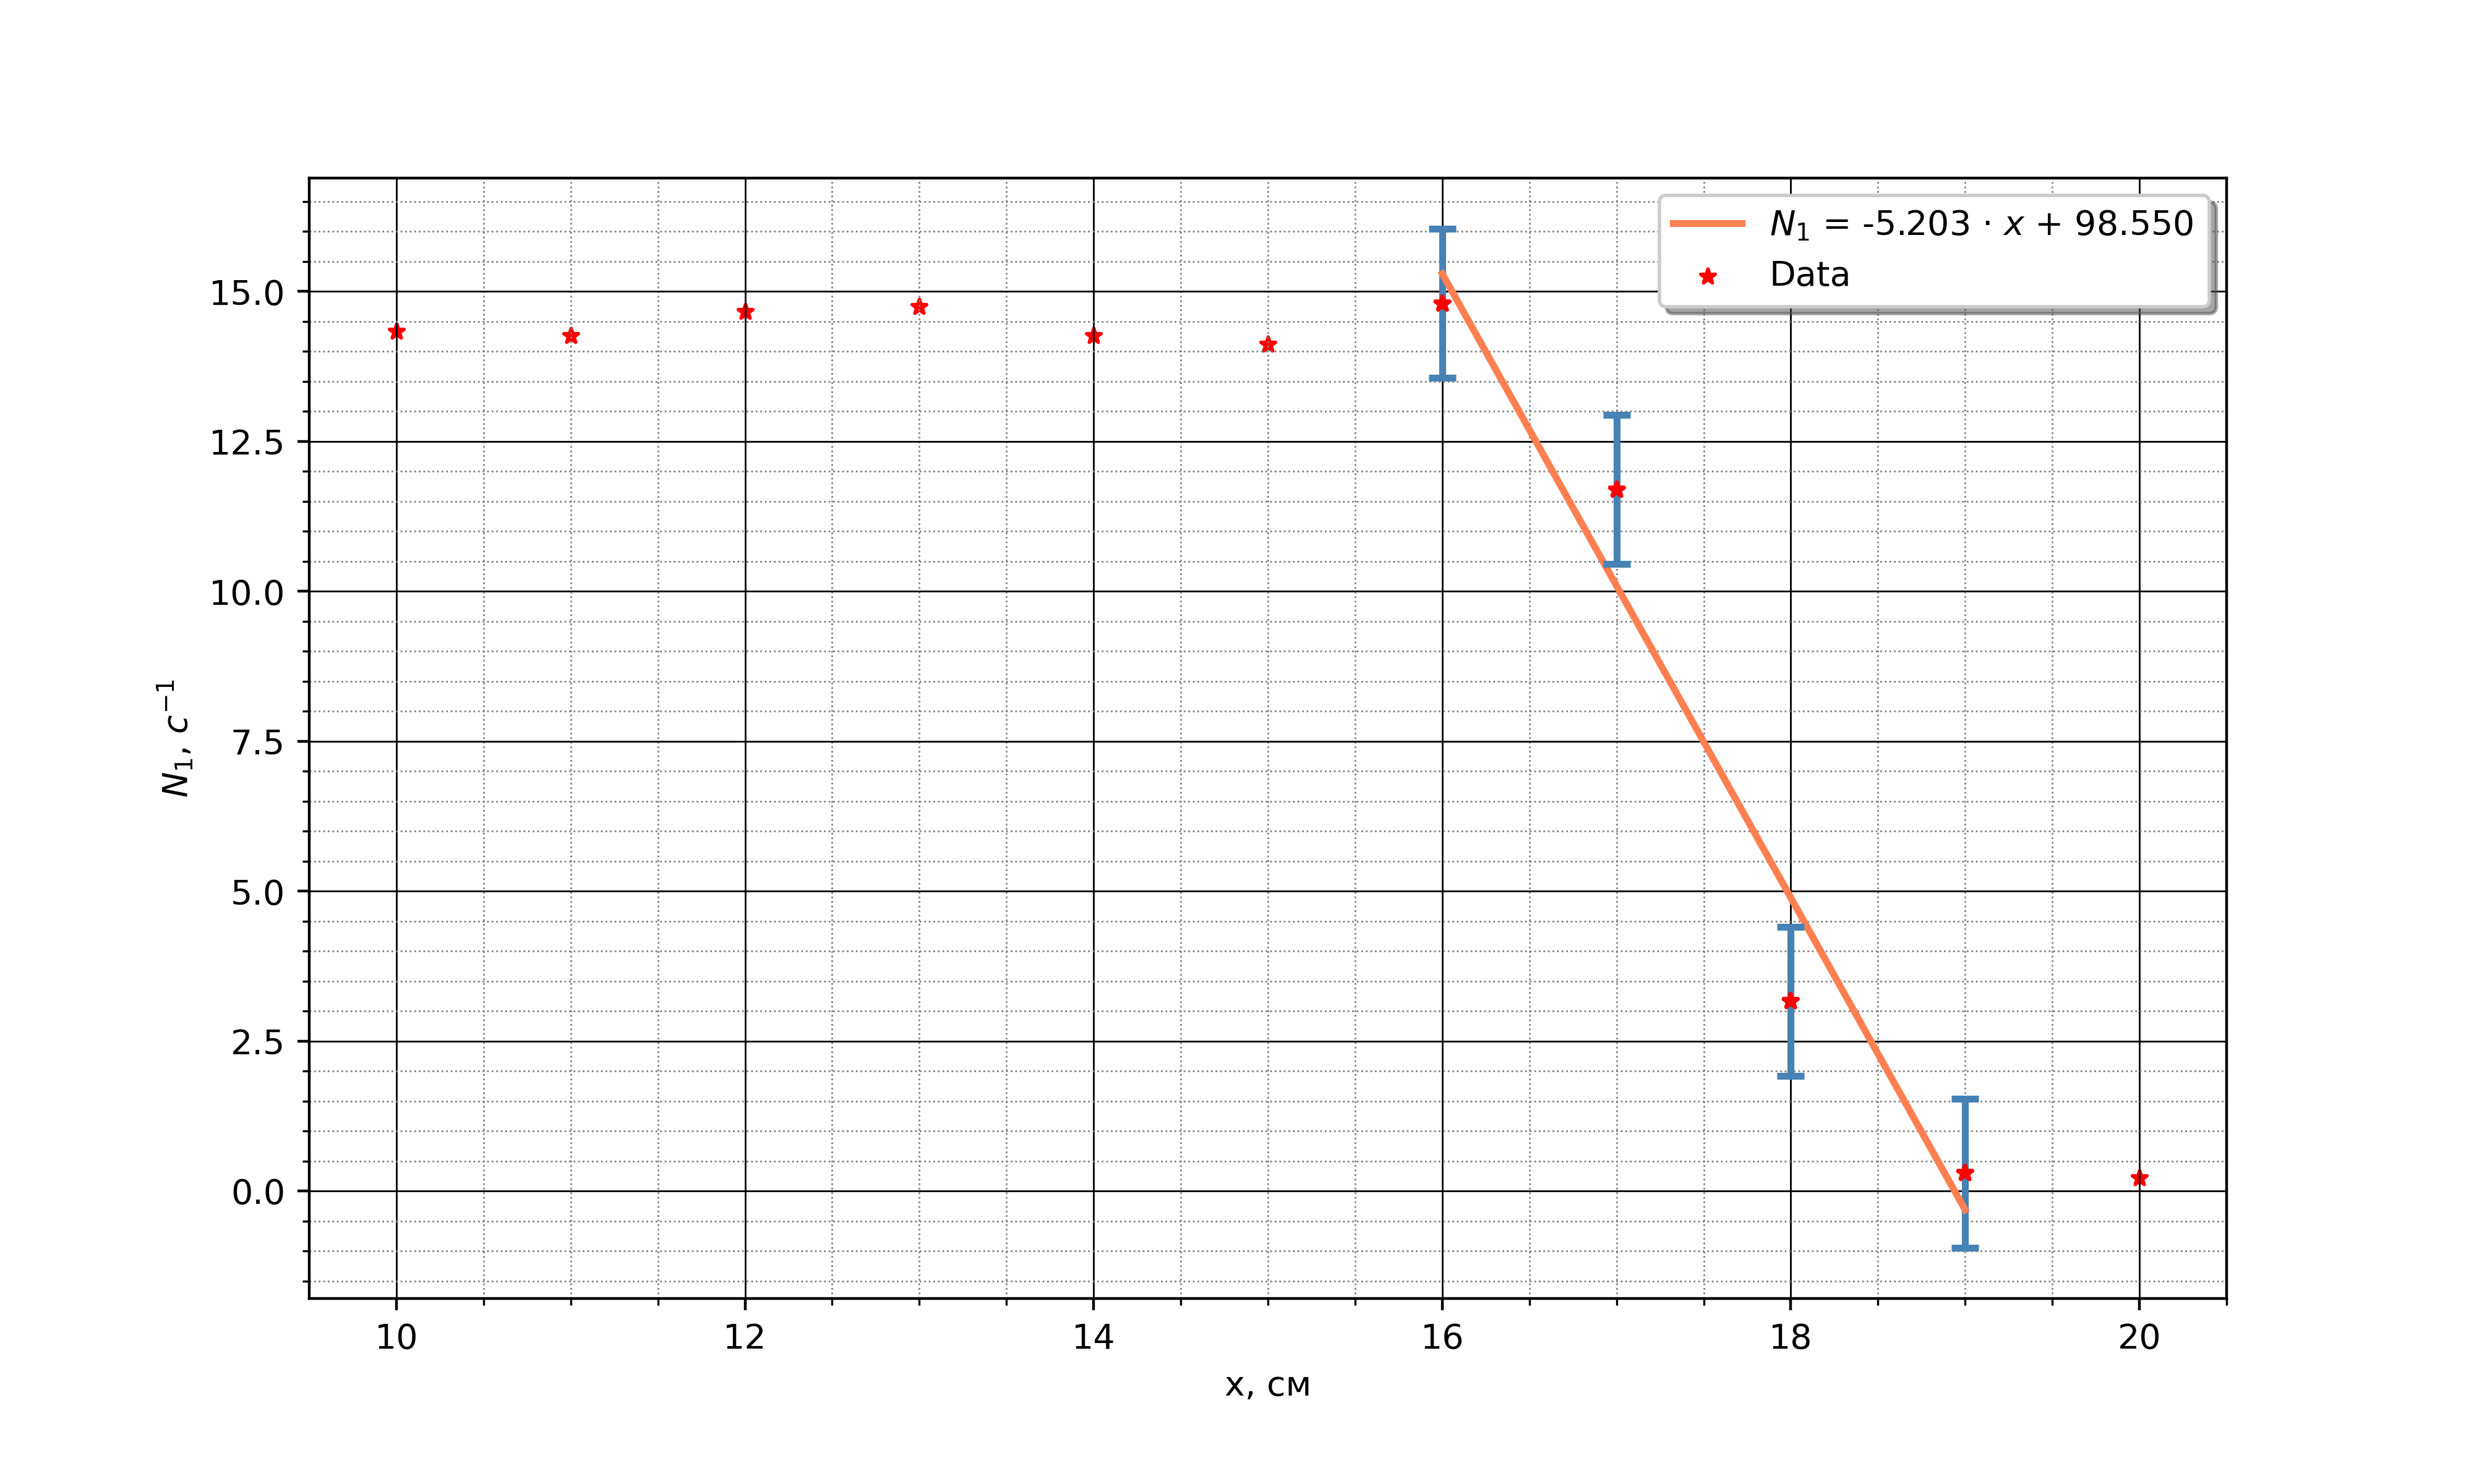
\includegraphics[scale = 0.8]{gr1.png}
        \caption{График зависимости $N_1(x)$}
        \label{gr1}
        \end{center}
    \end{figure}


    \item 
    Мы сделали фит точек в узком диапазоне в районе перегиба. Найдем экстраполируемый и средний пробег. 

    $$R_э = b/a \approx 18.94 \pm 3.9 [мм] (\pm \; 20.6 \%)$$
    $$R'_{э} = \rho \cdot R_{э} = 2.45 \pm 0.50\; г/см^2 $$

    Средняя длина пробега $R_{ср} \approx 17.5 \pm 1.0 \; мм$ $R'_{ср} = R_{ср} \cdot \rho  = 2.26 \pm 0.47 \; г/см^3$ 

    \item Оценим энергию этих альфа-частиц:
    
    $$E_{э} \approx 3.88 \pm 0.79 \; МэВ \;\;\;\;\;\;\; E_{ср} \approx 3.68 \pm 0.76 \; МэВ$$

\end{enumerate}



\subsection{Ионизационная камера}

\begin{enumerate}
    \item Включим установку, запишем нулевое показание табло.


    \item Включим питание ионизационной камеры. Проведем предварительные опыты. Откачаем камеру ток должен уменьшаться.
    
    
    \item Снимем зависимость тока от давления и занесем в таблицу 2:

    \begin{table}[h]
        \centering
        \caption{}
        \label{t1}
        \begin{tabular}{|c||c|c|c|c|c|c|c|c|}
            \hline
            $I$, пА&5& 72& 160& 239& 328 &424& 517& 626  \\ \hline
            $P$, Па &1333.22& 7999.32& 14665.42& 21331.52& 27997.62& 34663.72& 41329.82& 47995.92 \\ \hline
            \hline
            $I$, пА&840& 949& 1024& 1036& 1021& 1013& 1000&725 \\ \hline
            $P$, Па& 61328.12& 67994.22& 74660.32& 81326.42& 87992.52& 94658.62& 101324.72& 54662.02 \\ \hline
        \end{tabular}
    \end{table}


    \item Построим зависимость $I(P)$ на рис. \ref{gr2} и сделаем линейный фит

    \begin{figure}[H]
        \begin{center}
        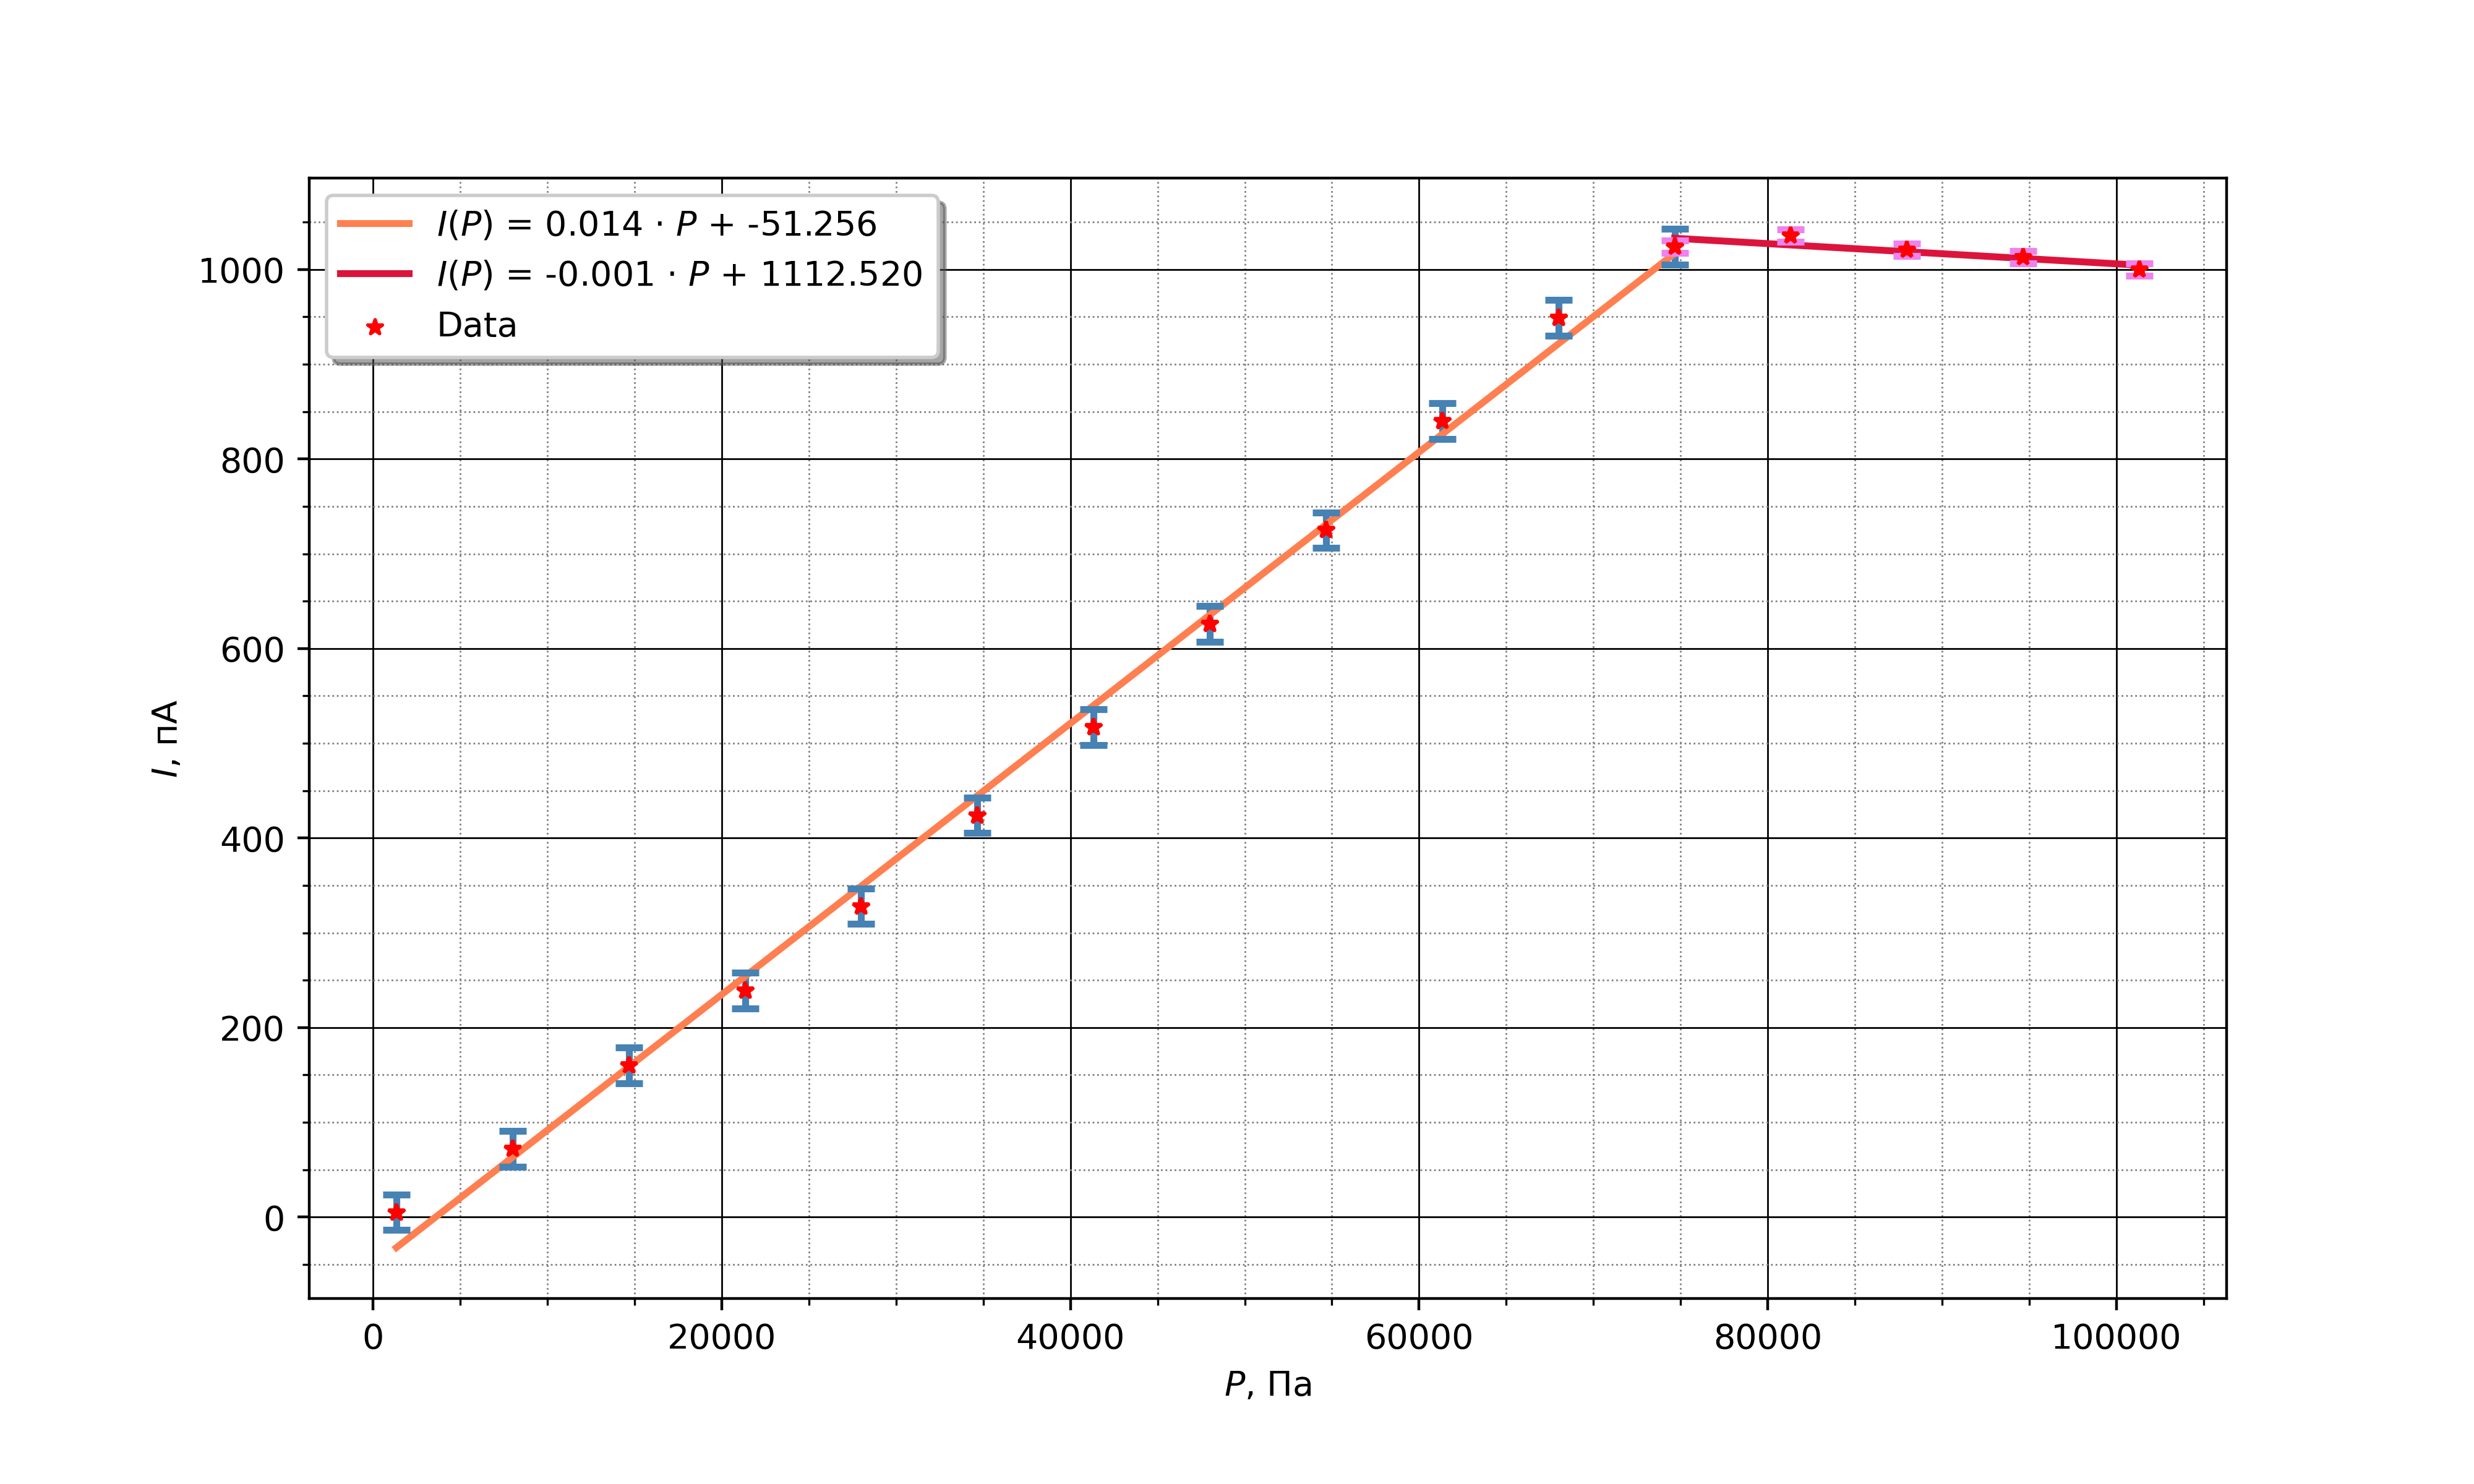
\includegraphics[scale = 0.8]{gr2.png}
        \caption{График зависимости $ I(P)$}
        \label{gr2}
        \end{center}
    \end{figure}

    
    \item Найдем точку пересечения прямых $P_0$:

    $$P_0 = \frac{b_2 - b_1}{a_1 - a_2} \approx 75700.24 \pm 2754.65 \; [Па] \; (\pm 3.6 \; \%)$$


    \item Зная , что при P = 760 Торр T = 300 K, через пропорцию найдем:

    $$R = (r_2-r_1) \cdot \frac{P_0}{P} \cdot \frac{T_0}{T} = 6.81 \pm 0.24 \; см$$
    $$R' = (8.8 \pm 0.3) \cdot 10^{-3} \; г/см^2$$


    \item Оценим энергию альфа-частиц:
    $$E = \left ( \frac{R}{0.32} \right ) \approx 8.79 \pm 0.03 \; МэВ$$
\end{enumerate}



\subsection{Сцинтилляционный счетсчик}

\begin{enumerate}
    \item Включим пересчетную устанвоку и выпрямитель. Проверим установку: проведем счет при атмосферном давлении 
    откачаем камеру, посмотрим, что все работает.


    \item Опыт будем проводить при напускании воздуха в камеру. Данные занесем в таблицу 3:
    
    \begin{table}[h]
        \centering
        \caption{}
        \label{t1}
        \begin{tabular}{|c||c|c|c|c|c|c|c|c|}
            \hline
            N& 3785& 3248&2265&1284&428&95&21&7 \\ \hline
            $P$, Па &1333.22& 7999.32& 14665.42& 21331.52& 27997.62& 34663.72& 41329.82& 47995.92 \\ \hline
        \end{tabular}
    \end{table}


    \item Построим зависимость N(P) на рис. \ref{gr3}
    
    \begin{figure}[H]
        \begin{center}
        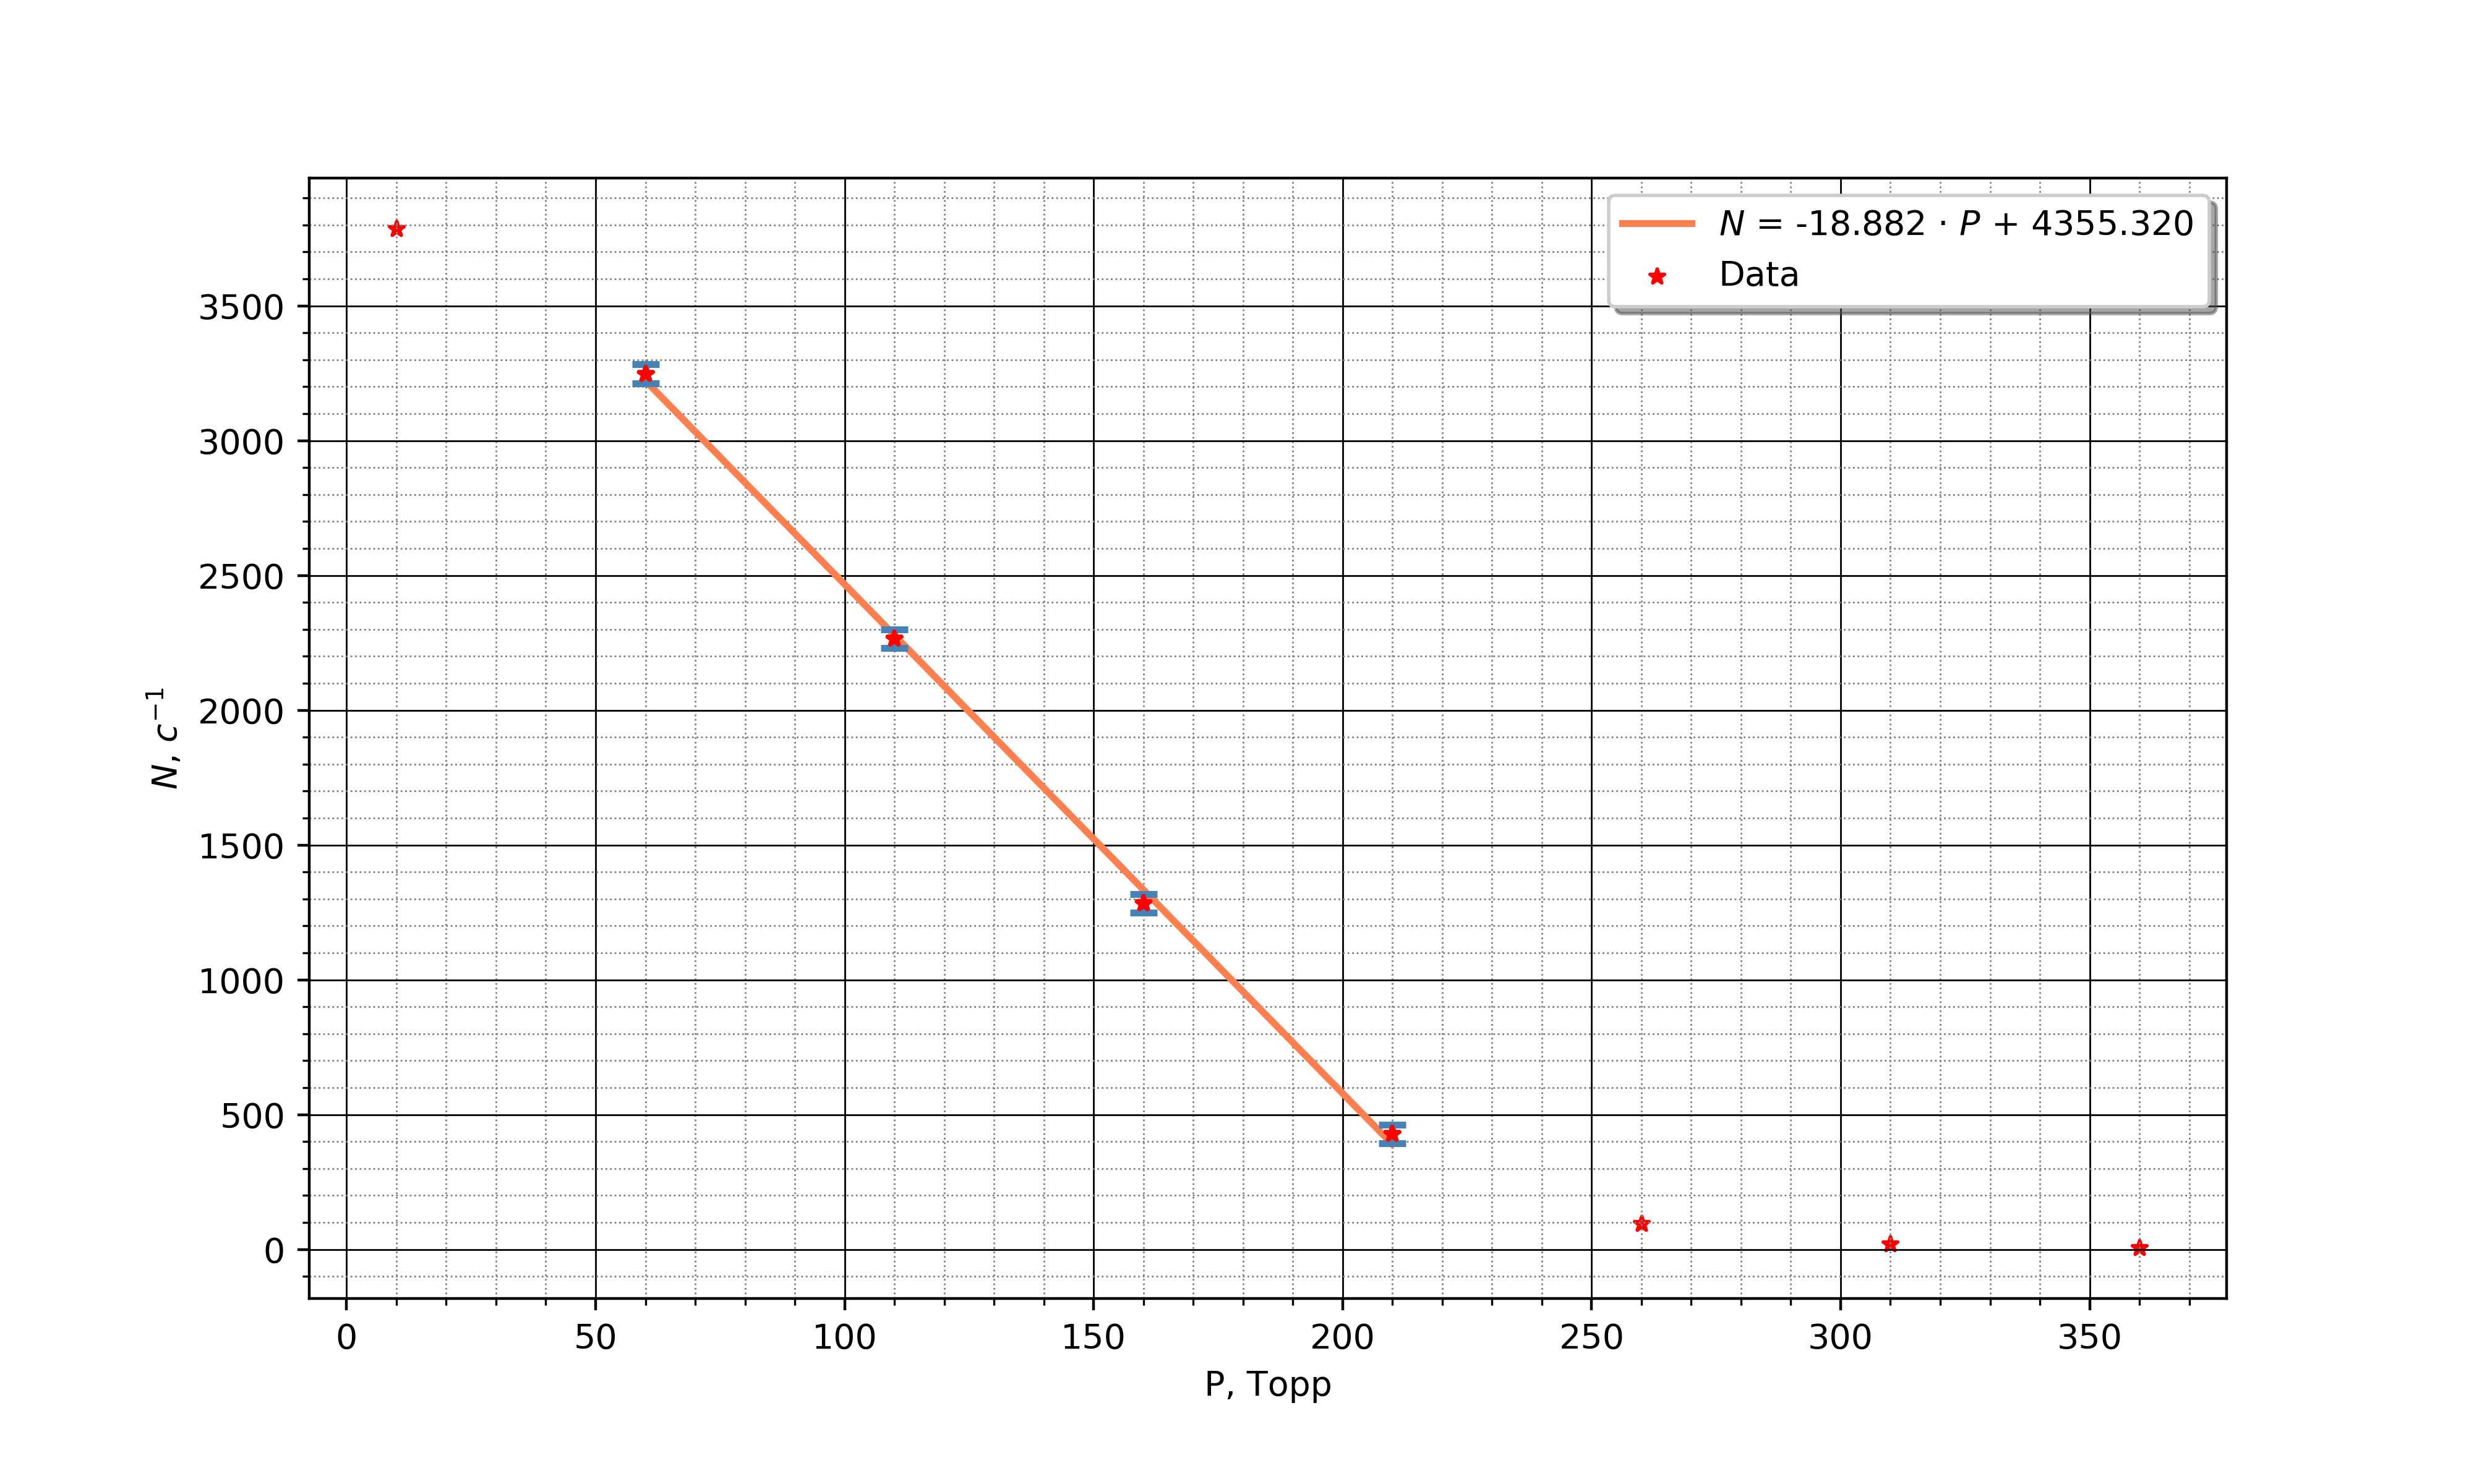
\includegraphics[scale = 0.8]{gr3.png}
        \caption{График зависимости $ N(P)$}
        \label{gr3}
        \end{center}
    \end{figure}

    \item По графику (рис. \ref{gr3}) определим экстраполируемое давление и среднее:
    
    $$P_э = b/a \approx 230.66 \pm 6.33 \; [Торр] \; (\pm \; 2.7 \%)$$
    $$P_{ср} \approx 150 \pm 10 Торр$$

    \item Найдем пробегпо формуле $R = \frac{P}{760\; [Торр]} \cdot 9 \; [см]$
    
    $$R_э = 2.73 \pm 0.08 \; см \;\;\;\;\;\;\;\;\;\; R'_э = (3.53 \pm 0.09) \cdot 10^{-3} \; [г/см^2]$$
    $$R_{ср} = 1.78 \pm 0.05 \; см \;\;\;\;\;\;\;\;\;\; R'_{ср} = (2.30 \pm 0.09) \cdot 10^{-3} \; [г/см^2]$$


    \item Определим энергию:
    
    $$E_{э} \approx 4.95 \pm 0.14 \; МэВ \;\;\;\;\;\;\; E_{ср} \approx 3.72 \pm 0.10 \; МэВ$$
\end{enumerate}



\section{Вывод}

В работе измерен проьбег альфа-частиц от источника $^{239}Pu$ тремя способами: с помощью торцевой счетсчика Гейгера и
ионизационной камеры и сцинтилляционного счетсчика, также определили энергию альфа-частиц. 



\end{document}